% Created 2021-09-27 Mon 12:01
% Intended LaTeX compiler: xelatex
\documentclass[letterpaper]{article}
\usepackage{graphicx}
\usepackage{grffile}
\usepackage{longtable}
\usepackage{wrapfig}
\usepackage{rotating}
\usepackage[normalem]{ulem}
\usepackage{amsmath}
\usepackage{textcomp}
\usepackage{amssymb}
\usepackage{capt-of}
\usepackage{hyperref}
\setlength{\parindent}{0pt}
\usepackage[margin=1in]{geometry}
\usepackage{fontspec}
\usepackage{svg}
\usepackage{cancel}
\usepackage{indentfirst}
\setmainfont[ItalicFont = LiberationSans-Italic, BoldFont = LiberationSans-Bold, BoldItalicFont = LiberationSans-BoldItalic]{LiberationSans}
\newfontfamily\NHLight[ItalicFont = LiberationSansNarrow-Italic, BoldFont       = LiberationSansNarrow-Bold, BoldItalicFont = LiberationSansNarrow-BoldItalic]{LiberationSansNarrow}
\newcommand\textrmlf[1]{{\NHLight#1}}
\newcommand\textitlf[1]{{\NHLight\itshape#1}}
\let\textbflf\textrm
\newcommand\textulf[1]{{\NHLight\bfseries#1}}
\newcommand\textuitlf[1]{{\NHLight\bfseries\itshape#1}}
\usepackage{fancyhdr}
\pagestyle{fancy}
\usepackage{titlesec}
\usepackage{titling}
\makeatletter
\lhead{\textbf{\@title}}
\makeatother
\rhead{\textrmlf{Compiled} \today}
\lfoot{\theauthor\ \textbullet \ \textbf{2021-2022}}
\cfoot{}
\rfoot{\textrmlf{Page} \thepage}
\renewcommand{\tableofcontents}{}
\titleformat{\section} {\Large} {\textrmlf{\thesection} {|}} {0.3em} {\textbf}
\titleformat{\subsection} {\large} {\textrmlf{\thesubsection} {|}} {0.2em} {\textbf}
\titleformat{\subsubsection} {\large} {\textrmlf{\thesubsubsection} {|}} {0.1em} {\textbf}
\setlength{\parskip}{0.45em}
\renewcommand\maketitle{}
\author{Houjun Liu}
\date{\today}
\title{Retroviruses}
\hypersetup{
 pdfauthor={Houjun Liu},
 pdftitle={Retroviruses},
 pdfkeywords={},
 pdfsubject={},
 pdfcreator={Emacs 28.0.50 (Org mode 9.4.4)}, 
 pdflang={English}}
\begin{document}

\tableofcontents



\section{Retroviruses}
\label{sec:org820560f}
\textbf{Viruses that have the ability to intergrate into the chromosomes of the
host cell}

\subsection{Retroviruses, infection}
\label{sec:org3cab6fd}
Normal \href{KBhBIO101ViralInfection.org}{KBhBIO101ViralInfection}
infection stuff happen, but then\ldots{}

\begin{itemize}
\item As the virus is uncoated, it uses an enzyme called "reverse
transcriptaese" to turn ssRNA to cDNA, and finally into dsDNA
(template strand DNA).
\item And, ready for this? The virus then uses an enzyme called
\textbf{intergraese} to thread the viral dsDNA into the cell's normal
nucleaus
\end{itemize}

A bonus for HIV (which is a Retrovirus) --- it utilities \textbf{protease} to
cut HIV's polyproteins into individual parts ready for budding.

\subsection{Retroviruses, Late Stage}
\label{sec:org89a91de}
The proviral region (the part that makes virus) newly inserted to the
cell's DNA is transcribed slowly when normal
\href{KBhBIO101CentralDogma.org}{KBhBIO101CentralDogma} comes across
it to synthesize proteins. In this case, this virus would spread through
cell duplication

When the cell is undergoing
\href{KBhBIO101CellLifecycle.org}{KBhBIO101CellLifecycle}, the
proviral area is replicated and exported as usual, making descendents of
the cell also have the proviral region. This property makes these
viruses especially hard to get rid of, which is why we still can't cure
HIV.

\noindent\rule{\textwidth}{0.5pt}

To make these activities happen, the virus needs two enzymes ---
\textbf{Reverse Transcriptaese} + \textbf{Intergraese}

\begin{itemize}
\item \textbf{Reverse Transcriptase}

\begin{itemize}
\item Transcript RNA to double-stranded RNA
\item Take double-stranded RNA to turn into DNA
\end{itemize}

\item \textbf{Integrase}

\begin{itemize}
\item Force insert the DNA into the genome of the host cell
\end{itemize}
\end{itemize}

\begin{figure}[htbp]
\centering
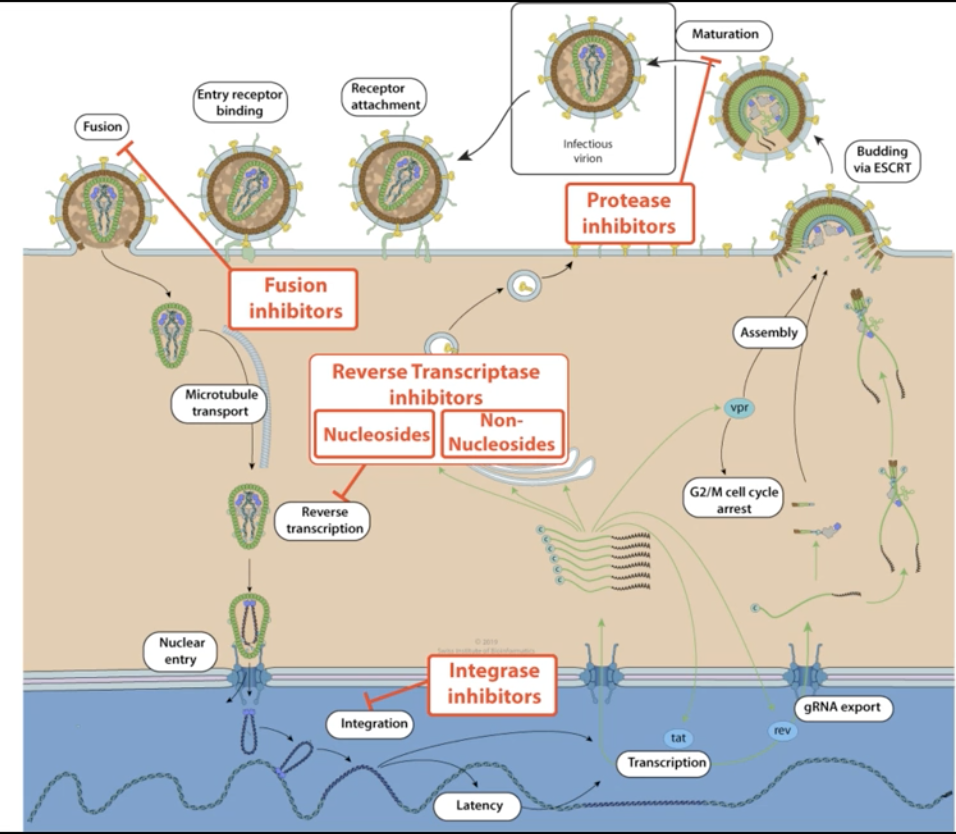
\includegraphics[width=.9\linewidth]{Screen Shot 2020-10-12 at 11.22.35 PM.png}
\caption{Screen Shot 2020-10-12 at 11.22.35 PM.png}
\end{figure}

\noindent\rule{\textwidth}{0.5pt}

\subsection{Preventing Retroviruses}
\label{sec:org6c178bc}
There are a few different drugs that prevent a few different steps of
the retroviral infection process

\begin{itemize}
\item Prevent \href{KBhBIO101ViralEntry.org}{KBhBIO101ViralEntry} \texttt{gp120},
\texttt{gp41}, \texttt{CCR5}
\item Prevent reverse transcription --- turn viral ssRNA to dsDNA \texttt{RT}
\item Prevent intergration via \textbf{intergrease} \texttt{IN}
\item Prevent viron maturation (namely, \textbf{protease} function) \texttt{PR}
\end{itemize}

\begin{figure}[htbp]
\centering
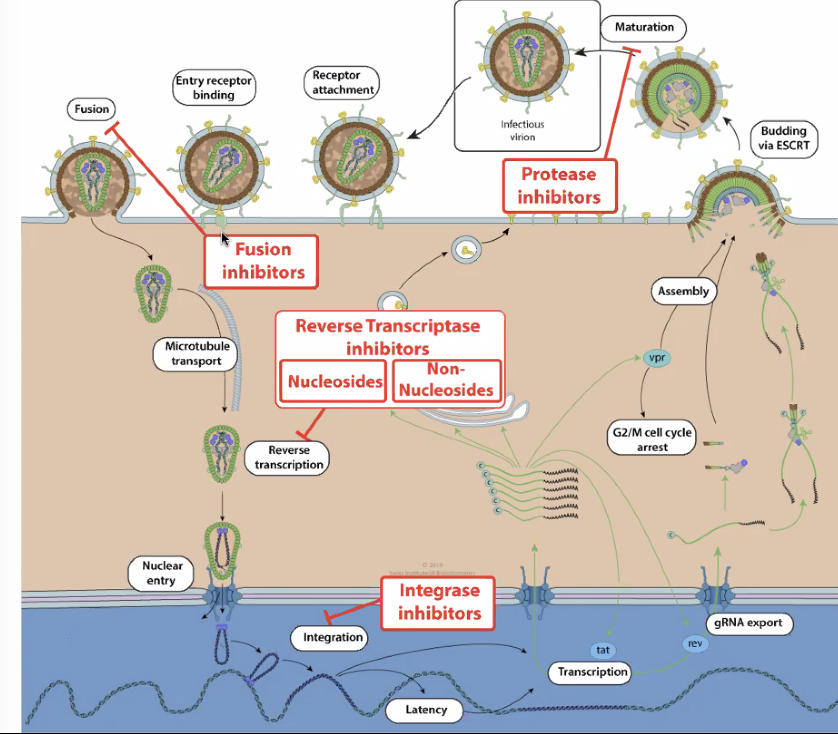
\includegraphics[width=.9\linewidth]{stophiv.png}
\caption{stophiv.png}
\end{figure}

Most advanced treatment: HAART (Highly-Active Anti-Retroviral Therapy)

\begin{itemize}
\item Cocktail drug works together for inhibition
\item Two drugs to stop intergration, one to stop protease (viron
maturation)
\item Could develop resistance
\end{itemize}
\end{document}
